\documentclass[a4paper]{article}

\usepackage{geometry}
\geometry{a4paper, margin=1in}
\usepackage{graphicx}
\usepackage{float}
\usepackage{listings}
\usepackage{xcolor}
\usepackage[utf8]{inputenc}

\lstset{
    basicstyle=\ttfamily\small,
    breaklines=true,
    frame=single,
    language=C++,
    keywordstyle=\color{blue},
    commentstyle=\color{green!50!black},
    stringstyle=\color{red}
}

\begin{document}

\title{Operating Systems Lab Assignment: Thread-Safe Data Structures}
\author{Jonathan Ross}
\date{October 19, 2025}
\maketitle

\section{Introduction}
This report documents the implementations and analyses for the thread-safe data structures lab
assignment, covering thread-safe queue and stack implementations, Producer-Consumer and
Undo-Redo use cases, and additional exercises.

\section{Exercise 1: Thread-Safe Queue and Stack}
\lstinputlisting[language=C++]{exercise1.cpp}
\textbf{Explanation}: In both classes, a lockguard locks the mutex in every method, creating a critical section that serializes access to the internal data structure. This locking prevents race conditions, enabling the ThreadSafeQueue to safely coordinate producer/consumer messages and the ThreadSafeStack to correctly manage undo/redo history.

\textbf{Analysis}: The mutex provides mutual exclusion, forcing any thread to block and wait if another thread is already accessing the data. Consumers terminate only after a pop fails and an atomic counter confirms all messages have been produced, guaranteeing no work is missed.

\textbf{Screenshot}: Include a screenshot of compiling and running exercise1.cpp.
\begin{figure}[H]
    \centering
    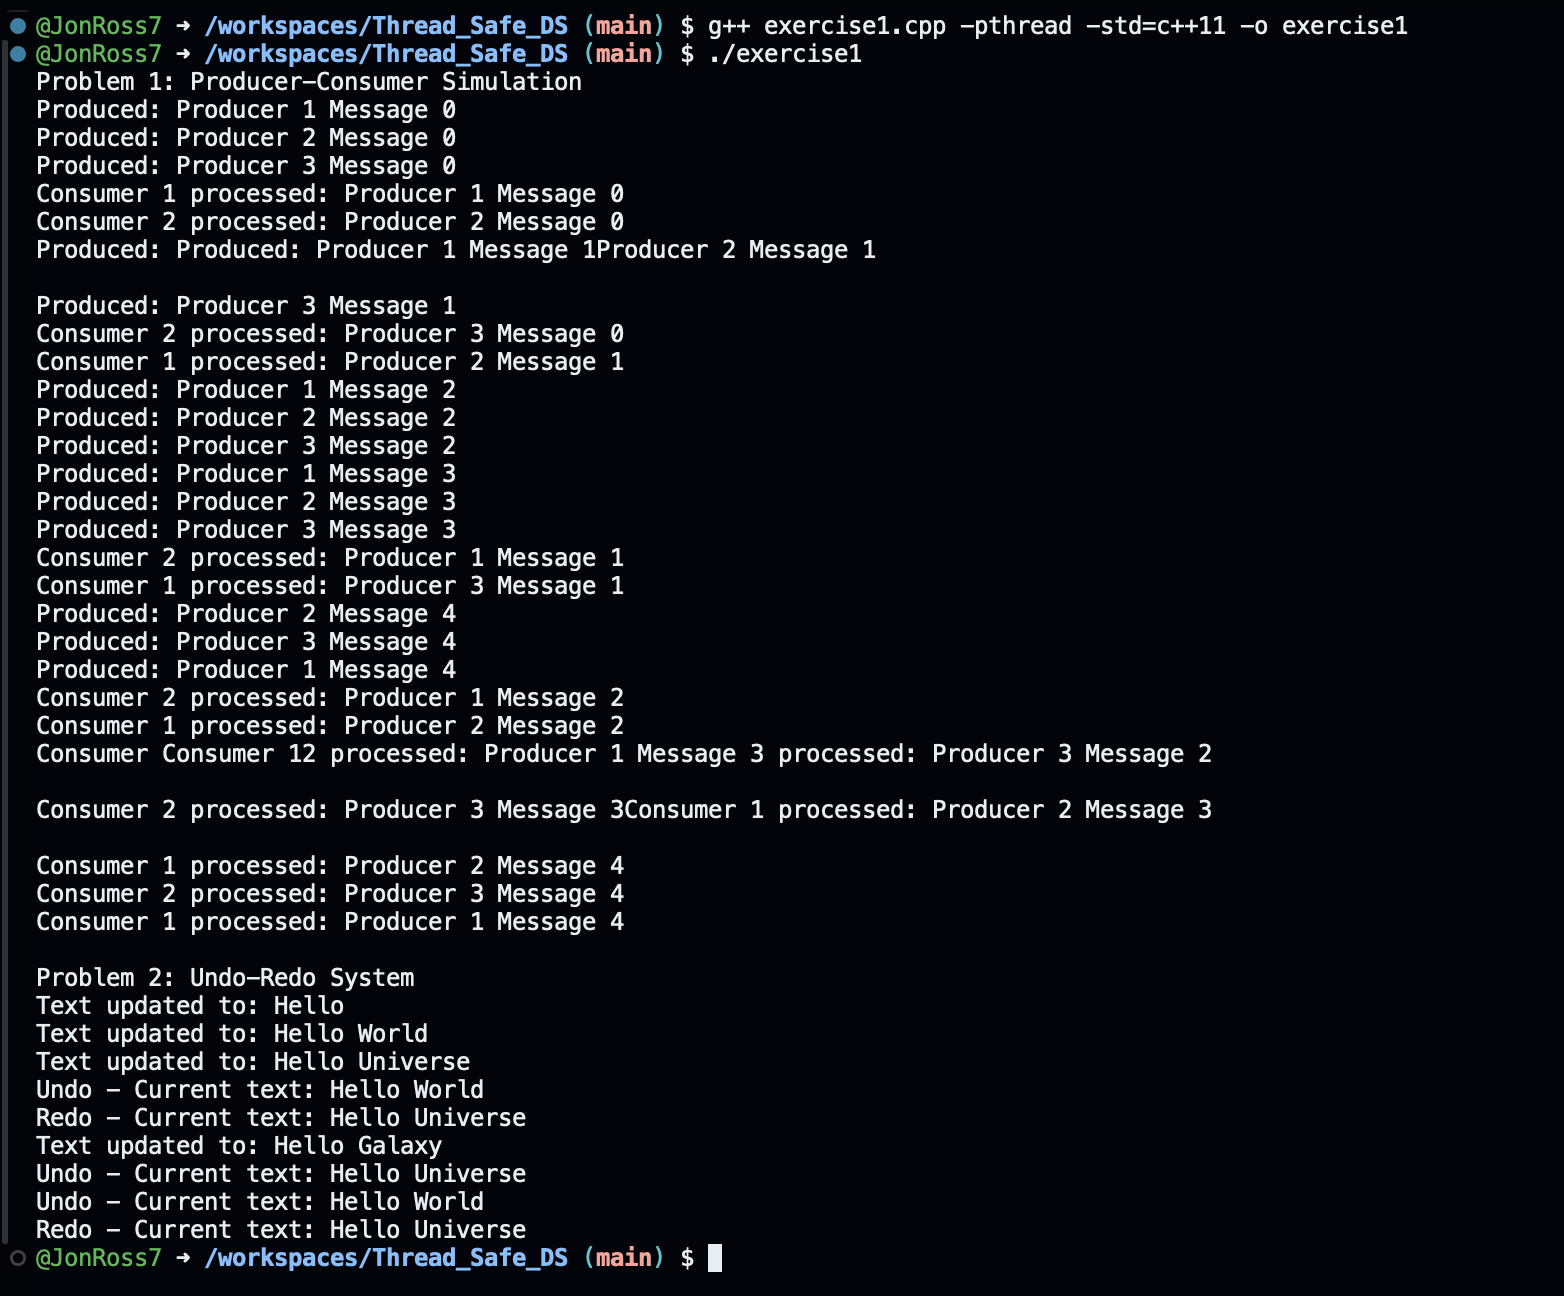
\includegraphics[width=\textwidth]{exercise1.png}
    \caption{Compilation and execution of exercise1.cpp}
\end{figure}

\section{Exercise 3: Thread-Safe Priority Queue}
\lstinputlisting[language=C++]{priorityQueue.cpp}
\textbf{Explanation}: The ThreadSafePriorityQueue ensures thread safety by using a lockguard to lock its mutex in every method, which serializes access and prevents race conditions. This locking protects the internal priority queue, allowing it to correctly maintain order so that pop operations always remove the highest-priority element, even when multiple threads are pushing and popping simultaneously.

\textbf{Analysis}: Concurrent push and pop operations are serialized by the mutex, meaning only one thread can modify the priority queue at any given time. While thread scheduling makes the order of operations non-deterministic, the pop thread is always guaranteed to receive the highest-priority item that is currently in the queue at the exact moment it acquires the lock.

\textbf{Screenshot}: Include a screenshot of compiling and running priorityQueue.cpp.
\begin{figure}[H]
    \centering
    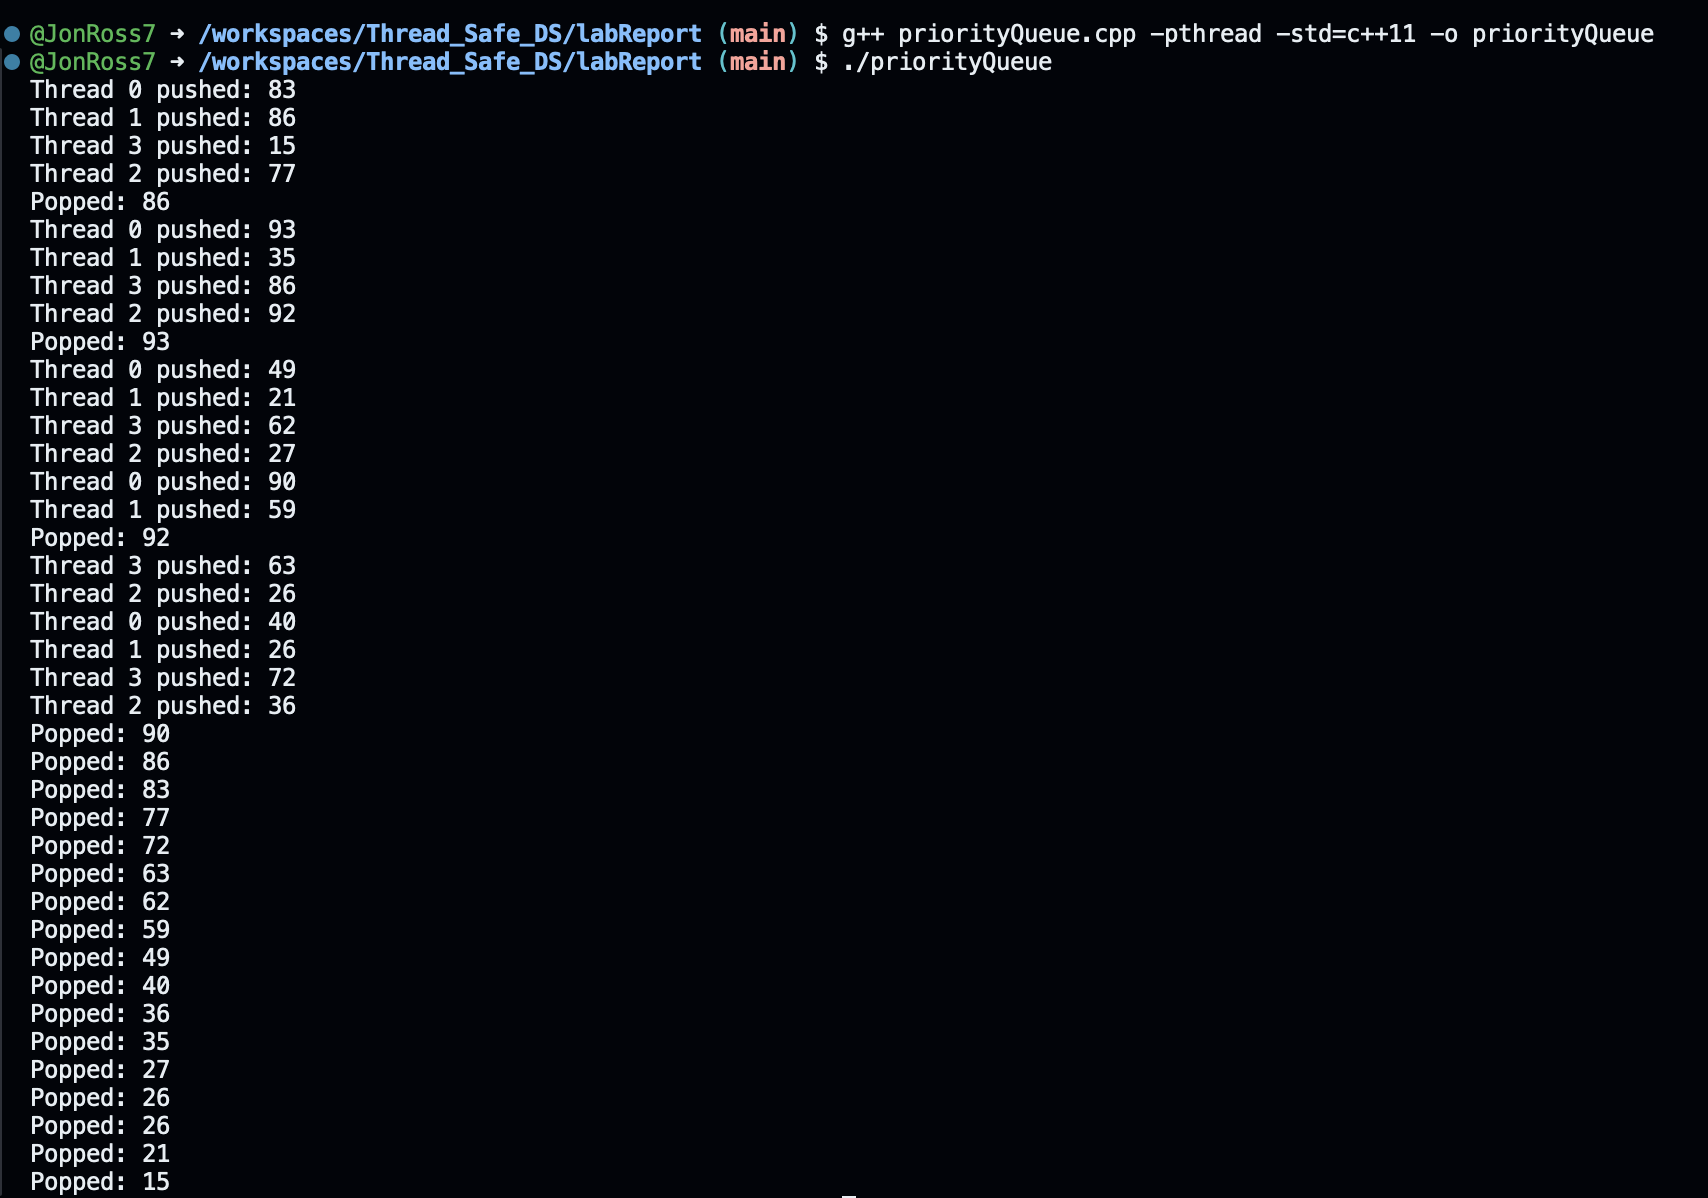
\includegraphics[width=\textwidth]{exercise3.png}
    \caption{Compilation and execution of priorityQueue.cpp}
\end{figure}

\section{Exercise 4: Thread-Safe Circular Buffer}
\lstinputlisting[language=C++]{circularBuffer.cpp}
\textbf{Explanation}: Condition variables allow threads to efficiently block and wait for a specific condition instead of spinning in a loop. A thread waits on the condition, which atomically unlocks the mutex and puts the thread to sleep. Another thread then uses notifyOne to wake the waiting thread after it changes the condition.

\textbf{Analysis}: The ThreadSafeQueue from Exercise 1 was unbounded and used only a mutex, which forced consumers to "busy-wait" by repeatedly trying to pop from an empty queue. This ThreadSafeCircularBuffer is bounded and uses condition variables to make threads wait when the buffer is full or empty, which is far more efficient as it eliminates busy-waiting entirely.

\textbf{Screenshot}: Include a screenshot of compiling and running circularBuffer.cpp.
\begin{figure}[H]
    \centering
    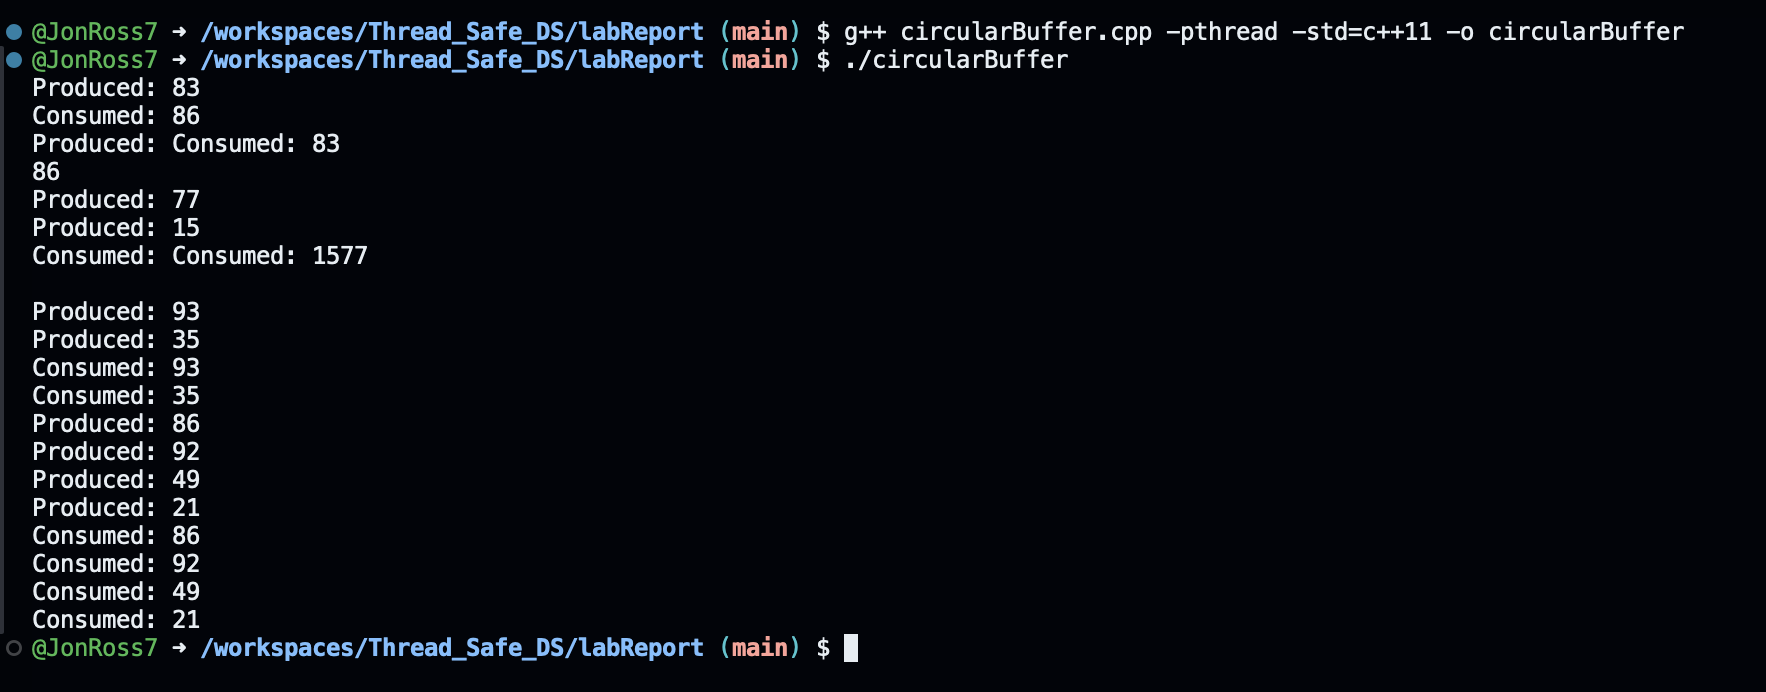
\includegraphics[width=\textwidth]{exercise4.png}
    \caption{Compilation and execution of circularBuffer.cpp}
\end{figure}

\section{Exercise 5: Thread-Safe Deque}
\lstinputlisting[language=C++]{threadSafeDeque.cpp}
\textbf{Explanation}: The main challenge is that operations on opposite ends don't inherently conflict, but operations on the same end or on an empty deque do create race conditions. This implementation uses a single, coarse-grained mutex that locks the entire deque for every operation, which solves the problem simply but creates a performance bottleneck by serializing all access, even non-conflicting ones.

\textbf{Analysis}: Concurrent operations on the deque are fully serialized because the single mutex locks the entire data structure for every method. This "coarse-grained" lock effectively prevents all race conditions, but it also creates a performance bottleneck by forcing even non-conflicting operations to wait for each other instead of running in parallel.

\textbf{Screenshot}: Include a screenshot of compiling and running threadSafeDeque.cpp.
\begin{figure}[H]
    \centering
    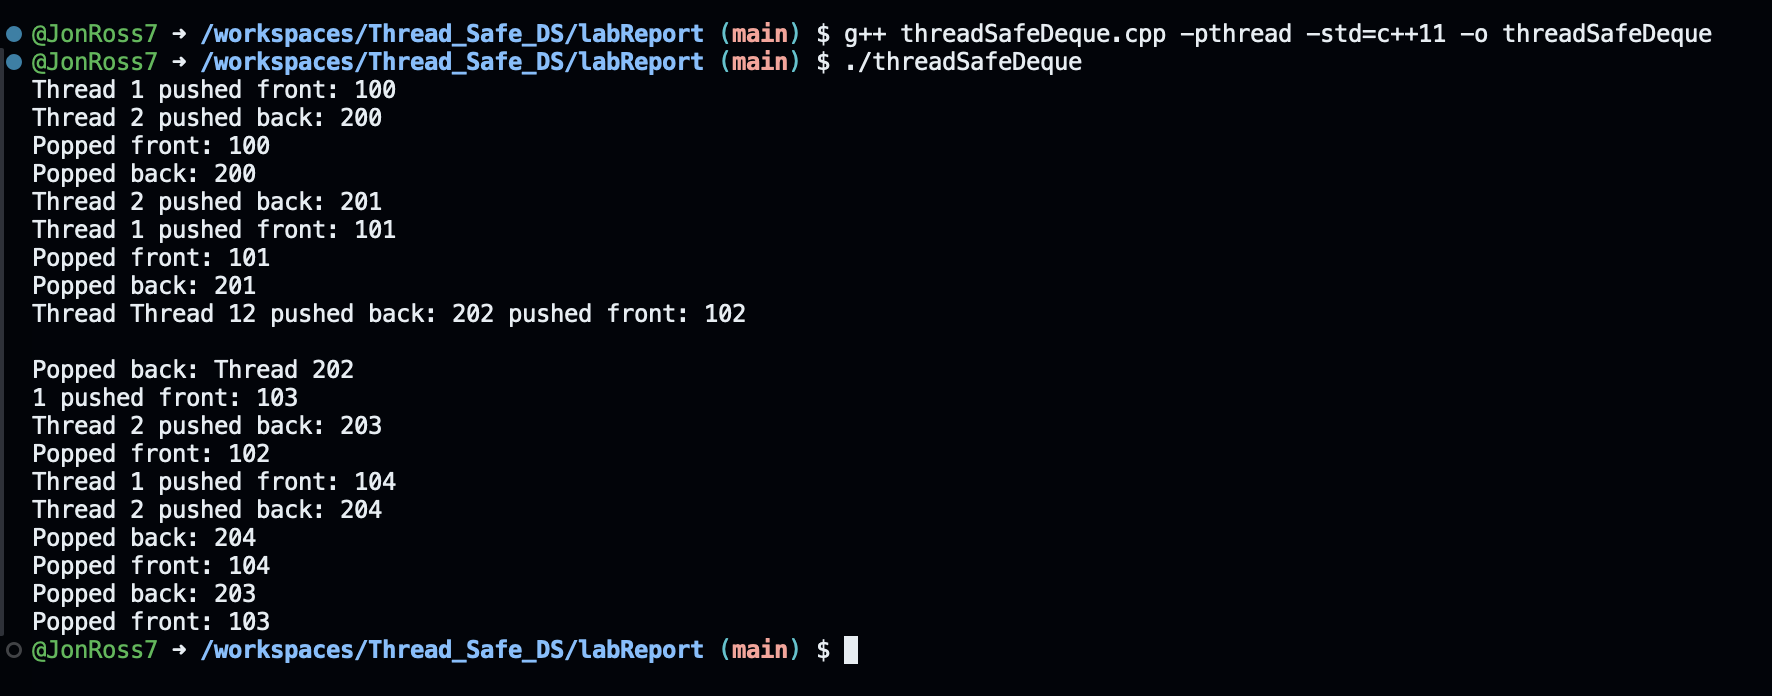
\includegraphics[width=\textwidth]{exercise5.png}
    \caption{Compilation and execution of threadSafeDeque.cpp}
\end{figure}

\section{Exercise 6: Thread-Safe Linked List}
\lstinputlisting[language=C++]{threadSafeLinkedList.cpp}
\textbf{Explanation}: The main challenge is that list operations like pushFront are not atomic. Instead, they involve multiple steps. If two threads execute these steps at the same time, they could read the same head value, and one thread's update would be lost, corrupting the list. This implementation uses a single, coarse-grained mutex to lock the entire list, which serializes all access and prevents these race conditions but also creates a bottleneck, as even non-conflicting operations are forced to wait.

\textbf{Analysis}: Thread safety is achieved using a single, coarse-grained mutex that locks the entire list for every operation, which simply and effectively prevents all race conditions. The major performance consideration is that this lock serializes all access, creating a bottleneck that limits scalability, as only one thread can operate on the list at a time, even for non-conflicting operations.

\textbf{Screenshot}: Include a screenshot of compiling and running threadSafeLinkedList.cpp.
\begin{figure}[H]
    \centering
    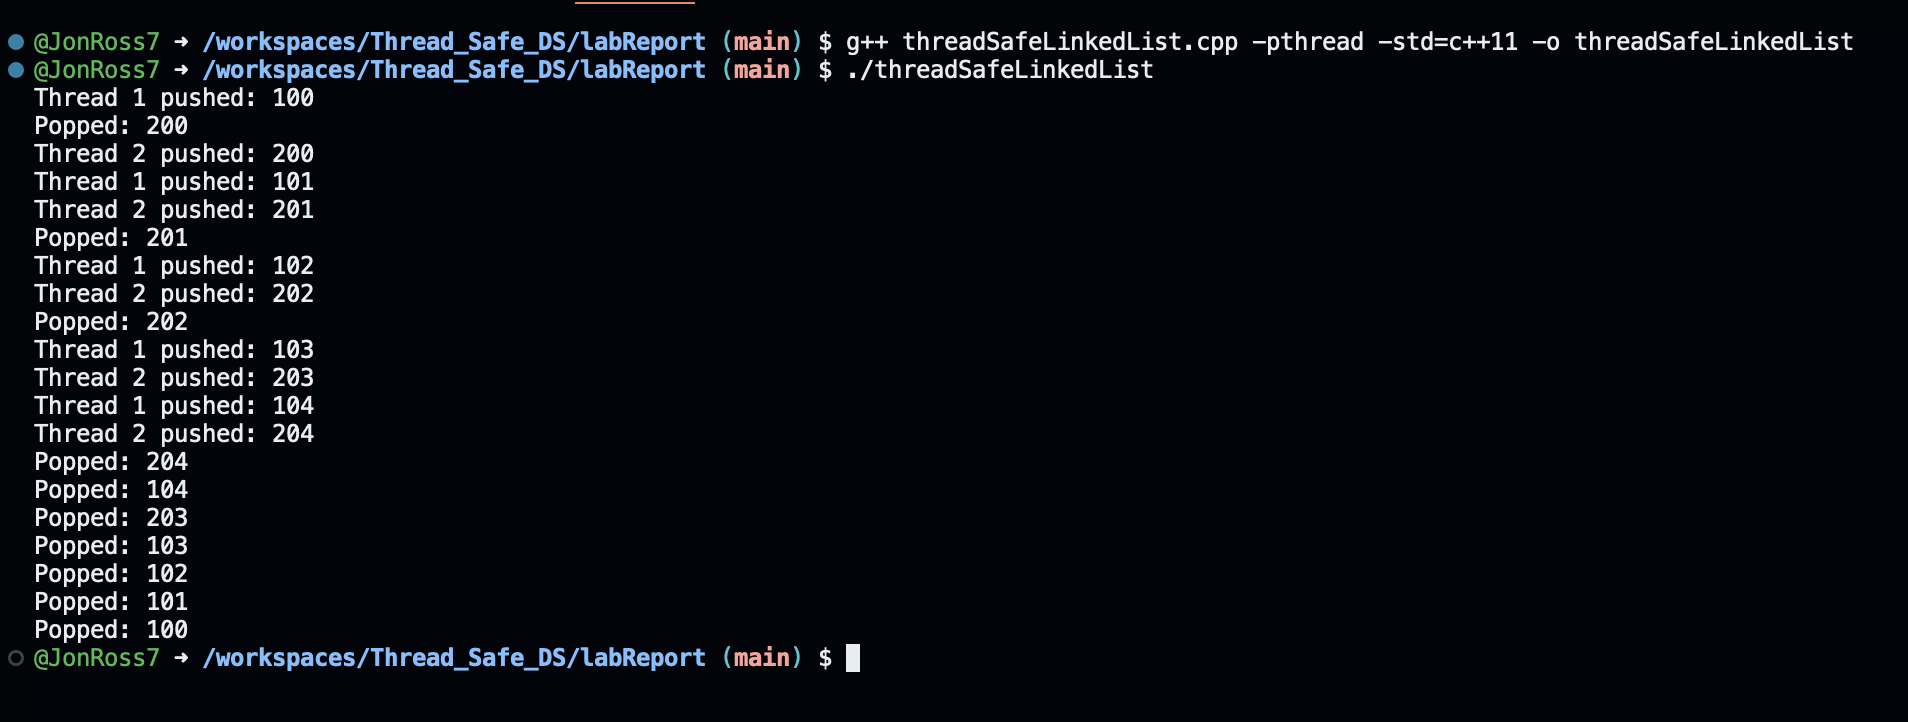
\includegraphics[width=\textwidth]{exercise6.png}
    \caption{Compilation and execution of threadSafeLinkedList.cpp}
\end{figure}

\end{document}